\section{Design}

As described in our motivation, there are two major aspects to STEAK’s design.  The first is the subsystem for securely and automatically managing keys.  We refer to this subsystem as AutoKey.  The second is the protocol for sending and receiving emails, called Secure Message Request Protocol (SMRP).  SMRP relies on AutoKey to ensure the sender and receiver have the appropriate keys in place before communicating.

\subsection{Architecture}
Our design assumes Alice and Bob both have sets of trusted endpoints that run loosely-synchronized clocks, and that each endpoint can access its user’s personal cloud storage account for hosting hard state across sessions.  Additionally, we assume Alice and Bob's endpoints can run code in execution and resource contexts outside of the web browser (such as in a VM).

There are four components to STEAK, beyond cloud storage and endpoint devices (Figure 1). The first is the STEAK endpoint code, which runs separately from the browser.  It performs key management, session management, caching, cloud storage access, cryptographic operations, and UI proxying. The second is the webmail UI, which differs from a conventional webmail UI only in that it issues its RPCs to the locally-hosted endpoint code instead of a remote webmail server.  These two components are intentionally separated for practical reasons, because at the time of this writing there is no way to perform cryptography inside the browser without exposing the user to a multitude of Javascript-based attacks, such as code injection, XSS, and inter-tab information leakage.

The third is the STEAK server, which helps the endpoints discover when the user has new mail, assists with backwards compatibility.  It also serves copies of users’ public keys, certificates, and storage signatures, which are mirrored by one or more metadata repositories (the fourth component).  Metadata repositories are not required for correct execution since they host redundant information, but using one or more of these increases the number of servers Mal must compromise to trick Alice and Bob.

The Alice’s endpoint, STEAK server, and metadata repositories work together to implement AutoKey for her.  Alice and Bob’s STEAK servers, cloud storage, and endpoints work together to implement SMRP.  Figure~\ref{fig:overview} shows how this manifests in inter-component communications.

\begin{figure}[h!]
\centering
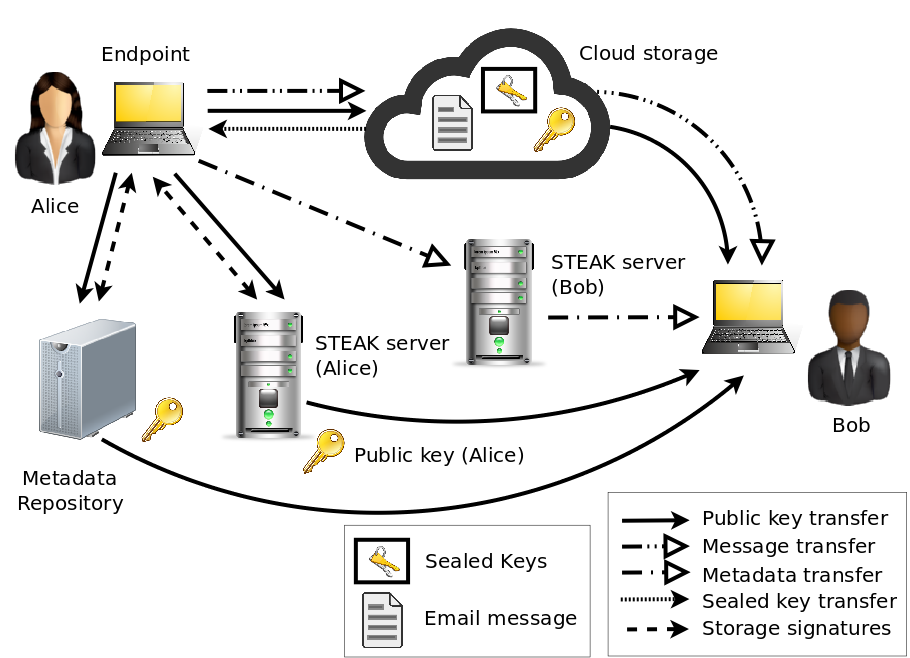
\includegraphics[width=0.5\textwidth]{figures/overview}
\caption{\it Overview of the STEAK architecture, and various data flows that must take place before Alice sends a message to Bob.  Solid-head arrows are part of the AutoKey process.  Unfilled-head arrows are part of the SMRP process.}
\label{fig:overview}
\end{figure}


In AutoKey, each user is given an account public/private key pair, a storage public/private key pair, and one or more signing public/private key pairs.  The private keys are stored encrypted with the user’s password, and only decrypted when the device is running a session.  The account and signing public keys are made available in the form of certificates signed by the account private key.  The use for each key pair is listed in Table~\ref{tab:keypairs}.

\begin{table*}[ht!]
\begin{tabular}{ | l | p{14cm} |}
\hline
\textbf{Key Pair Name} & \textbf{Usage} \\
\hline
Account key pair & Certifying and revoking other public keys. \\
Storage key pair & Sealing/unsealing and signing cloud-hosted data.  Used for message confidentiality and state CIA. \\
Signing key pair & Signing email messages and attachments.  Used for message integrity and authenticity. \\
\hline
\end{tabular}
\caption{\it Names and usages for a user`s key pairs used in STEAK`s AutoKey subsystem.}
\label{tab:keypairs}
\end{table*}


\subsubsection{Storage}
STEAK protects the contents of cloud storage from tampering by replicating cryptographic signatures.  Each file uploaded to cloud storage is sealed with the user’s storage private key for confidentiality.  STEAK organizes the files into a Merkel tree, such that each directory contains the signed hash of all of its children’s signed hashes.  Each hash is sealed by the storage private key, making external tampering from Mal evident.

Writing data is similar to two-phase commit.  A writer endpoint prepares to write by generating the new root signature, and replicating it to its STEAK server and all metadata repositories.  If they all authenticate and accept it, the writer uploads the data to cloud storage, and then broadcasts a signed success message.  The write completes when the STEAK server and metadata repositories acknowledge upon successful authentication.

Because reads and writes are serialized by the fact that the user does not use two endpoints simultaneously, the metadata repository only needs to store the last root signature it received.  To avoid timing out partway through writing, the endpoint splits large writes into smaller ones and commits them separately.

On read, the endpoint verifies the integrity of cloud storage by fetching the root signatures from these servers and comparing them to the one in cloud storage.  Because Mal cannot compromise all servers, and cannot compromise all channels, the reader will learn if Mal has tampered with a server if the signatures do not match.  These read and write protocols are executed by AutoKey to store trusted public keys in a tamper-evident way.

Given the threat Mal poses to the system, STEAK employs a fail-fast approach to handling storage faults.  This is because unavailability or inconsistencies discovered in cloud-hosted data (such as incorrect signatures) are assumed to be due to external interference from Mal.  This is a reasonable trade-off, because it alerts users and cloud storage operators to Mal’s presence.  We discuss in Section “Implementation” strategies to ensure the STEAK servers and metadata repositories have high availability.

Because only the user’s endpoints may write to the user’s cloud storage, STEAK is fundamentally a pull-based architecture.  Instead of sending data from Alice’s endpoint to Bob’s email server, Alice will write messages into her cloud storage, and Bob will download them later using SMRP.  This is a departure from SMTP, which we exploit to offer an “un-send mail” feature and to economically disincentivize spam mail by requiring the sender to pay for storage.

\subsubsection{Usability}
A user interacts with STEAK through the web browser, using the local endpoint as a web proxy.  The UI is stored as files in cloud storage and are signed by the storage private key.  The web browser fetches them through the endpoint so the endpoint can verify their authenticity and integrity before serving them over the local trusted RPC channel.  This prevents Mal from performing code injection attacks and XSS, and prevents Mal from learning private keys through side-channel attacks in the browser.

Before Alice or Bob can use STEAK, they must set up the endpoint code.  However, doing so does not impose a significant usability burden---it can be packaged into an app and made available from an endpoint-specific app store.  We discuss strategies to facilitate this initial step in section “Implementation.”  We assume in the following sections that the endpoints all run instances of the endpoint code in local VMs.

\subsection{Bootstrapping Trust}
Before Alice can use STEAK, she needs an account.  In creating one, she bootstraps AutoKey by establishing her public key and registration date with each component, populating her cloud storage with initial application state, and granting her endpoint permission to access to it.  She also establishes security questions and answers to be used to recover her private key, should she forget her password.

\begin{figure}[h!]
\centering
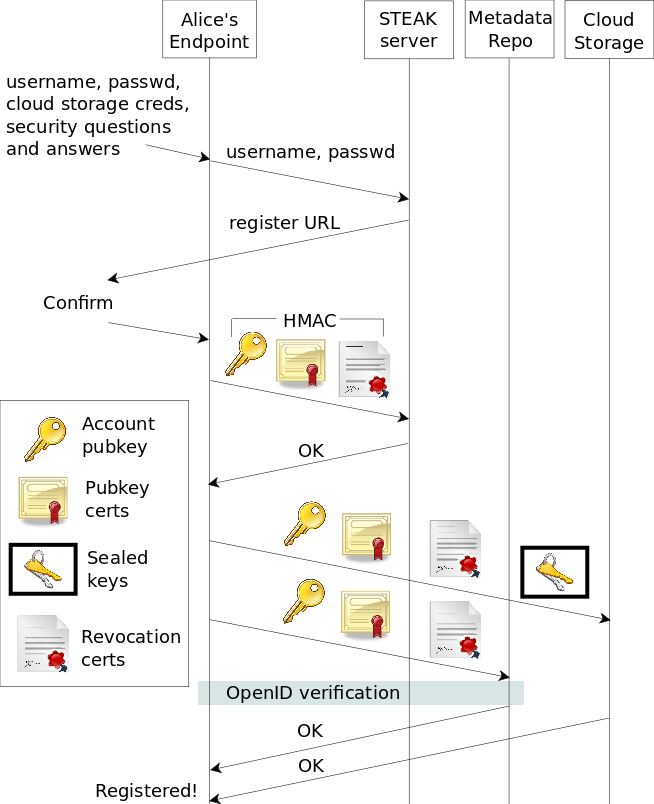
\includegraphics[width=0.5\textwidth]{figures/register}
\caption{\it The STEAK key registration protocol.}
\label{fig:register}
\end{figure}

To do so, her endpoint replicates her account public key and backs up her revocation certificate to more servers than Mal can compromise.  We assume that Mal cannot alter the behavior of the servers during the registration process; if the servers do not behave correctly, the registration fails (Figure~\ref{fig:register}).

From a usability standpoint, creating an account on the STEAK server is similar to doing so on a webmail server.  Alice begins by submitting a desired username and password to the STEAK server through the endpoint, as well as any number of hard-to-guess security questions and answers, and the identifier for an uncompromisable out-of-band channel to confirm the registration (e.g. a phone number or existing email address).  The STEAK-specific extra requirements are the authentication tokens needed to access her cloud storage, and her additional metadata repositories.

Once the information is entered, the endpoint uploads the username and password to the STEAK server, which replies with a one-time-use registration URL via the out-of-band channel.  Alice navigates to the URL to complete her registration.  Both the server and endpoint employ TLS-secured communication channels to prevent Eve from learning Alice’s password.  Once Alice confirms, the STEAK server remembers iterated salted hash of the out-of-band channel identifier, so Mal cannot easily learn it and so Alice can use it later to reset her password.

Once Alice’s account is created on the STEAK server, the endpoint sets up her keys and certificates.  It generates her public/private key pairs, and signs the storage and signing public keys with the account private key.  It then generates revocation certificates for the account and storage keys, as well as two public certificates---one for the signing key, and one for the storage key---that contain Alice’s username, the public key, the timestamp, and a nonce for uniqueness (“pubkey certs” in Figure~\ref{fig:register}).  It signs these certificate with the account private key.

It then proceeds to replicate the account public key and certificates to each server, using the STEAK server to vouch for her.  To upload them to the STEAK server, It generates an HMAC over them using the password as the shared secret.  Once the STEAK server validates and accepts them (remembering the nonce to prevent re-register attacks), the endpoint uploads them to each metadata repository.  The endpoint authenticates to each using OpenID protocol and Alice’s password, where the STEAK server acts as the OpenID provider.  The metadata repositories do not consider a revocation certificate to be in force until Alice activates it (see “Key Revocation”).

The endpoint finishes by populating Alice’s cloud storage with STEAK account state, using the authentication tokens she supplied at the beginning of the process.  It uploads her public key certificates as a world-readable files in cloud storage (for Bob to download later) as well as her revocation certificates and account public key (which are NOT encrypted).  It encrypts the private keys and cloud storage credentials using an authenticated symmetric key scheme, deriving symmetric keys from her salted password.  It also seals a copy of the storage private key with the answers to her security questions, so Alice can change her password without losing her data.  The endpoint uploads the security questions and sealed keys to cloud storage, seals the MACs and salts from the encryption with the password, and erases them from RAM, completing the registration and AutoKey bootstrap process.

\subsection{Session Management}
Once AutoKey is bootstrapped, Alice can use multiple endpoints to access her account transparently.  To do so, Alice simply enters her username and password, and the endpoint (via AutoKey) fetches her sealed storage private key, endpoint-specific sealed signing private key, and sealed cloud storage credentials.  If the device has never been used before, the endpoint generates a new signing key certificate and revocation certificate for it, seals the private key with the password, and distributes the certificates to the STEAK server and metadata repositories (which authenticate them with the account public key they obtained on registration).  The servers do not publish the revocation certificates until Alice signals them to do so.

Alice has the option to designate that the endpoint will be used for only one session (akin to a “This device is public” checkbox in webmail).  If so, the signing key will have an expiration date in the very near future, e.g. 30 minutes.

When Alice logs out or her session times out, the endpoint has AutoKey erase any secrets from RAM.  As a precaution, it also erases any data it cached data, and will erase cached data automatically if it restarts. Cached data is always sealed with one of Alice's public keys before being written to local storage, preventing Eve from breaking confidentiality via offline analysis.

\subsection{Key Distribution}
In AutoKey, Bob’s endpoint must learn Alice's account, storage, and signing public keys before he can communicate with her.  Once it has them, AutoKey puts them into his cloud storage, executing the two-phase write protocol so his other endpoints can securely and automatically fetch them later.  The challenges are in obtaining them for the first time in such a way that Eve and Mal cannot trick him into learning the wrong ones, and in revoking trust in them without also being tricked.

Bob’s endpoint will trust one of Alice’s public keys only if AutoKey can get unanimous agreement on the key’s value from each server that hosts them, and only if the key is not expired.  Similarly, AutoKey will check for an activated revocation certificate (see next section) if all servers agree on the same key, and the key is different from the currently trusted key.  This strategy works under our threat model because without Alice’s password, Mal is not powerful enough to send the wrong key on every channel, or change it to every server.

While Bob trusts the keys, AutoKey periodically checks to see if it Alice’s servers have changed them.  Because the account public key and storage public key do not change as often as the signing key (see the next section), it will check the account key at most once per session.  However, it will check the storage and signing public keys every time Bob composes a message to Alice.

To advertise her keys, Alice’s STEAK address is a well-formed email address that indicates her username, her cloud storage provider, her STEAK server, and any metadata repositories that host her keys.  We use the character ‘\^’ to separate them---for example, Alice’s STEAK address might be alice\^cloudstorage.com\^keybackup.org@mail.net, indicating that her data is hosted at cloudstorage.com, her keys are replicated to keybackup.org, and her STEAK server is mail.net.  Each service makes both the keys and certificates available via canonical URLs derived from the username and the service name.  Bob’s endpoint has AutoKey use TLS-secured channels to fetch copies from each service.

In the event that some of Alice’s services are unreachable, AutoKey continues to trust Bob’s copies of Alice’s public keys even if there is disagreement among the online servers.  This is to prevent Mal from weakening the system with denial-of-service attacks.  In practice, Alice’s services run on highly-available infrastructure, so unreachability problems are expected to be rare and transient.

\subsection{Key Revocation}


\begin{figure}[h!]
\centering
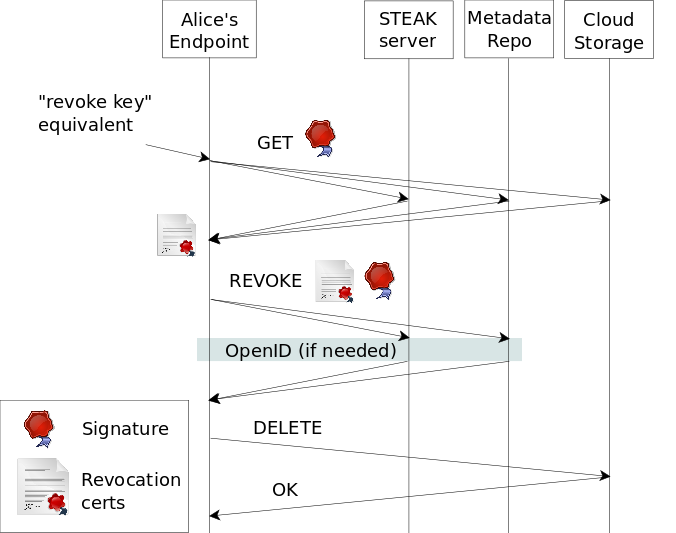
\includegraphics[width=0.5\textwidth]{figures/revoke}
\caption{\it The STEAK key revocation protocol.}
\label{fig:revoke}
\end{figure}

Inevitably, AutoKey will need to revoke Alice’s keys for her.  When Alice removes access permission from a trusted endpoint device, AutoKey revokes its signing key.  When she changes or resets her password, AutoKey revokes and regenerates her keys by default because the reason for doing so may be due to a password compromise.

Revoking a signing key is a matter of activating its stored revocation certificate (Figure~\ref{fig:revoke}).  To do so, AutoKey first obtains it by downloading it from each the servers, using a request signed by the account private key.  It also gets a copy from cloud storage.  At least one of the servers will reply with the correct revocation certificate, since Mal cannot compromise all of them under our threat model.

AutoKey then re-uploads it in a signed request to the servers, indicating that the should publish it.  The servers erase the old public key certificate on successful verification, and AutoKey removes it from cloud storage.  Then, when Bob contacts Alice next, his endpoint will detect the key discrepancy, discover the revocation certificate, and stop trusting the old signing key.

If Eve compromises Alice’s password, she will be able to read her incoming messages, and messages sent to others.  If Mal compromises Alice’s password, she can do anything with the account.  To regain control, Alice resets her password, effectively re-registering her account and re-bootstrapping AutoKey using registration protocol described earlier (but with two small differences described below).  As before, we assume that Mal cannot alter the behavior of the servers during re-registration.

Unlike with first-time registration, the STEAK server requires Alice to submit the same out-of-band communication channel as she did before.  Also, AutoKey sets a flag while uploading new public key information to ask for a reply containing the old revocation certificate.  It also obtains the copy uploaded earlier from cloud storage, and then executes a variant of the signing key revocation protocol to publish the revocation certificates for her account and storage keys.  The only differences are that the revocation certificates will be signed by the new account key, and that the servers will additionally verify the request with OpenID to ensure that it came from Alice (the only person who knows the new password).

When Alice logs in next, her endpoint “imports” her old account data by unsealing it with the old storage key and re-sealing it with the new storage key.  If Alice remembers her old password, her endpoint decrypts the old storage key automatically.  If she does not, her endpoint obtains the copy of the storage key sealed with the answers to her security questions, and prompts her for them to decrypt it.

Deleting an account is similar to revoking the keys.  The only difference in the process is that no new keys are generated.

\subsection{Sending, Receiving, and Un-Sending Email}
Once Alice and Bob have exchanged public keys with AutoKey, they communicate with SMRP, described in this section.  In SMRP, Alice sends Bob a message by sealing it with his public key, uploading it to her cloud storage, and making it world-readable. Bob’s endpoint downloads and decrypts it, sanitizes it, and serves it to Bob’s browser for him to read. The same principle applies to attachments, which in STEAK are sent as separate files to be downloaded.

If Bob expects email from Alice, he can search Alice’s cloud storage for new messages and fetch them.  The UI allows him to query individual contacts for new messages.

The challenge for Bob is to discover when Alice sent him an unsolicited message.  To address this in SMRP, Bob’s STEAK server acts as a notification service for new email.  Alice sends Bob's STEAK server a message metadata record, signed with her signing private key, that identifies herself as the sender and Bob as the recipient.  It serves as a hint to Bob that he has unsolicited mail, and contains a string of text sealed with Bob’s private key that identifies all of the message recipients, the subject, the human-readable names of the attachments, and the signature of the message body and each attachment.  This information is hidden from the STEAK server to provide end-to-end message CIA, and its small size makes it easy to store many of them.

When Bob accesses his email, his endpoint downloads the unread message metadata records from the server, stores them into his cloud storage, and sends a hint to the server that it can erase them.  Each of these message metadata records appear in Bob's UI as unread messages. The UI tells Bob the subject, recipients, and attachment names.

In SMRP, buffering message metadata records on the STEAK server is reasonable in practice. Bob’s endpoint will replicate them to cloud storage once it receives them, so the STEAK server can erase them once they have been passed on.  Because Bob only needs to learn the email addresses of the senders in order to scan their cloud storage for messages, the STEAK server only needs to remember the set of unique account names (the rest of the record can be dropped to save space at the cost of latency).  Since Bob can be expected to check his account frequently (once per day), it is unlikely that his message metadata records or the email address set will consume too much space.  We discuss strategies to mitigate denial-of-service attacks in the next section.

When Bob opens an unread message from Alice, his endpoint downloads, decrypts, and verifies the authenticity and integrity of Alice's message body. Once verified, Bob reads it via the browser UI. To download an attachment, the endpoint streams it from Alice's cloud storage, verifies it, decrypts it, and delivers it to the UI as a file download.  As a performance optimization (and to assist automatic spam filtering), the endpoint prefetches message bodies as they are discovered.

By default, once Bob obtains a message’s body and attachments, his endpoint automatically replicates them to his cloud storage in order to keep them available regardless of Alice's subsequent actions.  This is important, because before Bob reads a message, Alice can delete the message body and attachments from her cloud storage.

Although this is an artifact of our pull-based architecture, SMRP offers the ability to “un-send” a message by erasing the body and attachments from cloud storage.  This allows Alice to withdraw messages sent in haste, or sent accidentally to unintended people.  Bob may figure out that she deleted it after sending it (i.e. he may receive a metadata record for a message that does not exist), but Alice may prefer this to having Bob reading the entire message.

\subsection{Searching, Tagging, and Filtering Email}
Beyond sending and receiving email, webmail users expect automatic spam filtering, the ability to organize messages and conversations, and the ability to search them.  In traditional webmail systems, this functionality resides on the server.  The challenge providing it in STEAK is in moving it to the endpoint to preserve confidentiality, but without compromising features.

Tagging messages is a matter of associating a given message with a bag of tags that Bob defines.  Bob’s endpoint incrementally builds an index that pairs each tag to a list of message metadata records (ordered by when they were tagged).  To search messages by tag, the endpoint fetches a page of the tag’s index, then the message metadata records in the page, and serves them to the UI.  The message metadata record identifies the message to download and render once Bob clicks on it.

Our strategy for searching is to have the endpoint incrementally build a search index as Bob reads messages, using an existing indexer.  The indices are updated and synchronized with cloud storage in the background as he opens and reads messages.  As a performance optimization, the endpoint lazily downloads the index in fixed-sized chunks as they are needed by the indexer.  The endpoint caches them through the session, and asynchronously replicates modified chunks.

Our strategy for filtering spam messages is to rely on an combination of a locally-trained classifier and sender blacklists.  Bob has the option of marking messages as spam and marking senders as spammers, in which case the endpoint feeds the message body into its local spam classifier and replicates the classifier’s new model parameters to cloud storage.  This allows the classifier to be used across endpoints, without revealing the model parameters.  If Bob marks a contact as a spammer, he revokes trust in its public key, and the endpoint will ignore future messages from it.

Using only a local spam filter is desirable for confidentiality.  The spam classifier model parameters can leak information about the contents of the messages they have classified, so it is important that Bob’s endpoint not share this information directly.  This is in contrast to webmail providers today, which learn to classify spam by monitoring many user accounts.  However, empirical tests suggest that existing local spam filters can achieve upwards of 98\% effectiveness in practice, suggesting that our strategy should not significantly impact usability if the endpoint code ships with a pre-trained classifier.

\subsection{Backwards Compatibility}
Because email is already a widely-used service, STEAK must remain backwards compatible with it to allow Alice and Bob to communicate with Charles, a user who relies on conventional email.  To do so, the STEAK server provides an SMTP/SMRP gateway that translates one protocol into the other.  The STEAK server has its own cloud storage to hold messages from Charles to serve to Alice via SMRP.  Alice’s messages to Charles are automatically routed through SMTP because Charles does not have a well-formed STEAK email address.

The gateway alone does not provide CIA guarantees.  If Charles wants a limited degree of CIA, STEAK offers one of two options that require a minimal change in his workflow.  First, if Charles uses PGP already, he will email Alice his public key, and then simply send encrypted messages via SMTP.  AutoKey obtains Charles’ public key from the email.  While this is less trustworthy than STEAK’s approach, it is often better than nothing because Mal has only one very short window of time to alter the public key.

If Charles does not use PGP, he must first agree with Alice on a shared secret out-of-band, assume that Mal does not compromise the STEAK server or the TLS CA server that vouches for its TLS public key.  To send her a message securely, he navigates to her STEAK server, enters the secret, and is served a webmail form for composing her a message.  STEAK makes the message available to Alice via SMRP.

In this mode, when Alice sends Charles a message via SMRP, the STEAK server sends Charles a URL instead of the message body.  When opened, the STEAK server gives him a specially-crafted HTML page that contains Alice’s ciphertext, a decryption algorithm in Javascript, and a secret submission form.  When Charles enters the secret, the page decrypts the message for him.
